% Options for packages loaded elsewhere
\PassOptionsToPackage{unicode}{hyperref}
\PassOptionsToPackage{hyphens}{url}
%
\documentclass[
]{article}
\usepackage{amsmath,amssymb}
\usepackage{lmodern}
\usepackage{iftex}
\ifPDFTeX
  \usepackage[T1]{fontenc}
  \usepackage[utf8]{inputenc}
  \usepackage{textcomp} % provide euro and other symbols
\else % if luatex or xetex
  \usepackage{unicode-math}
  \defaultfontfeatures{Scale=MatchLowercase}
  \defaultfontfeatures[\rmfamily]{Ligatures=TeX,Scale=1}
\fi
% Use upquote if available, for straight quotes in verbatim environments
\IfFileExists{upquote.sty}{\usepackage{upquote}}{}
\IfFileExists{microtype.sty}{% use microtype if available
  \usepackage[]{microtype}
  \UseMicrotypeSet[protrusion]{basicmath} % disable protrusion for tt fonts
}{}
\makeatletter
\@ifundefined{KOMAClassName}{% if non-KOMA class
  \IfFileExists{parskip.sty}{%
    \usepackage{parskip}
  }{% else
    \setlength{\parindent}{0pt}
    \setlength{\parskip}{6pt plus 2pt minus 1pt}}
}{% if KOMA class
  \KOMAoptions{parskip=half}}
\makeatother
\usepackage{xcolor}
\usepackage[margin=1in]{geometry}
\usepackage{color}
\usepackage{fancyvrb}
\newcommand{\VerbBar}{|}
\newcommand{\VERB}{\Verb[commandchars=\\\{\}]}
\DefineVerbatimEnvironment{Highlighting}{Verbatim}{commandchars=\\\{\}}
% Add ',fontsize=\small' for more characters per line
\usepackage{framed}
\definecolor{shadecolor}{RGB}{248,248,248}
\newenvironment{Shaded}{\begin{snugshade}}{\end{snugshade}}
\newcommand{\AlertTok}[1]{\textcolor[rgb]{0.94,0.16,0.16}{#1}}
\newcommand{\AnnotationTok}[1]{\textcolor[rgb]{0.56,0.35,0.01}{\textbf{\textit{#1}}}}
\newcommand{\AttributeTok}[1]{\textcolor[rgb]{0.77,0.63,0.00}{#1}}
\newcommand{\BaseNTok}[1]{\textcolor[rgb]{0.00,0.00,0.81}{#1}}
\newcommand{\BuiltInTok}[1]{#1}
\newcommand{\CharTok}[1]{\textcolor[rgb]{0.31,0.60,0.02}{#1}}
\newcommand{\CommentTok}[1]{\textcolor[rgb]{0.56,0.35,0.01}{\textit{#1}}}
\newcommand{\CommentVarTok}[1]{\textcolor[rgb]{0.56,0.35,0.01}{\textbf{\textit{#1}}}}
\newcommand{\ConstantTok}[1]{\textcolor[rgb]{0.00,0.00,0.00}{#1}}
\newcommand{\ControlFlowTok}[1]{\textcolor[rgb]{0.13,0.29,0.53}{\textbf{#1}}}
\newcommand{\DataTypeTok}[1]{\textcolor[rgb]{0.13,0.29,0.53}{#1}}
\newcommand{\DecValTok}[1]{\textcolor[rgb]{0.00,0.00,0.81}{#1}}
\newcommand{\DocumentationTok}[1]{\textcolor[rgb]{0.56,0.35,0.01}{\textbf{\textit{#1}}}}
\newcommand{\ErrorTok}[1]{\textcolor[rgb]{0.64,0.00,0.00}{\textbf{#1}}}
\newcommand{\ExtensionTok}[1]{#1}
\newcommand{\FloatTok}[1]{\textcolor[rgb]{0.00,0.00,0.81}{#1}}
\newcommand{\FunctionTok}[1]{\textcolor[rgb]{0.00,0.00,0.00}{#1}}
\newcommand{\ImportTok}[1]{#1}
\newcommand{\InformationTok}[1]{\textcolor[rgb]{0.56,0.35,0.01}{\textbf{\textit{#1}}}}
\newcommand{\KeywordTok}[1]{\textcolor[rgb]{0.13,0.29,0.53}{\textbf{#1}}}
\newcommand{\NormalTok}[1]{#1}
\newcommand{\OperatorTok}[1]{\textcolor[rgb]{0.81,0.36,0.00}{\textbf{#1}}}
\newcommand{\OtherTok}[1]{\textcolor[rgb]{0.56,0.35,0.01}{#1}}
\newcommand{\PreprocessorTok}[1]{\textcolor[rgb]{0.56,0.35,0.01}{\textit{#1}}}
\newcommand{\RegionMarkerTok}[1]{#1}
\newcommand{\SpecialCharTok}[1]{\textcolor[rgb]{0.00,0.00,0.00}{#1}}
\newcommand{\SpecialStringTok}[1]{\textcolor[rgb]{0.31,0.60,0.02}{#1}}
\newcommand{\StringTok}[1]{\textcolor[rgb]{0.31,0.60,0.02}{#1}}
\newcommand{\VariableTok}[1]{\textcolor[rgb]{0.00,0.00,0.00}{#1}}
\newcommand{\VerbatimStringTok}[1]{\textcolor[rgb]{0.31,0.60,0.02}{#1}}
\newcommand{\WarningTok}[1]{\textcolor[rgb]{0.56,0.35,0.01}{\textbf{\textit{#1}}}}
\usepackage{graphicx}
\makeatletter
\def\maxwidth{\ifdim\Gin@nat@width>\linewidth\linewidth\else\Gin@nat@width\fi}
\def\maxheight{\ifdim\Gin@nat@height>\textheight\textheight\else\Gin@nat@height\fi}
\makeatother
% Scale images if necessary, so that they will not overflow the page
% margins by default, and it is still possible to overwrite the defaults
% using explicit options in \includegraphics[width, height, ...]{}
\setkeys{Gin}{width=\maxwidth,height=\maxheight,keepaspectratio}
% Set default figure placement to htbp
\makeatletter
\def\fps@figure{htbp}
\makeatother
\setlength{\emergencystretch}{3em} % prevent overfull lines
\providecommand{\tightlist}{%
  \setlength{\itemsep}{0pt}\setlength{\parskip}{0pt}}
\setcounter{secnumdepth}{-\maxdimen} % remove section numbering
\ifLuaTeX
  \usepackage{selnolig}  % disable illegal ligatures
\fi
\IfFileExists{bookmark.sty}{\usepackage{bookmark}}{\usepackage{hyperref}}
\IfFileExists{xurl.sty}{\usepackage{xurl}}{} % add URL line breaks if available
\urlstyle{same} % disable monospaced font for URLs
\hypersetup{
  pdftitle={TP 2 Clasificacion},
  hidelinks,
  pdfcreator={LaTeX via pandoc}}

\title{TP 2 Clasificacion}
\author{}
\date{\vspace{-2.5em}}

\begin{document}
\maketitle

TP 2 Clasificacion. Tomas Palazzo y Axel Fridman

Cargamos las librerias

\begin{Shaded}
\begin{Highlighting}[]
\FunctionTok{library}\NormalTok{(}\StringTok{"ggplot2"}\NormalTok{)                  }
\FunctionTok{library}\NormalTok{(}\StringTok{"GGally"}\NormalTok{)}
\end{Highlighting}
\end{Shaded}

\begin{verbatim}
## Registered S3 method overwritten by 'GGally':
##   method from   
##   +.gg   ggplot2
\end{verbatim}

\begin{Shaded}
\begin{Highlighting}[]
\NormalTok{df }\OtherTok{=} \FunctionTok{read.csv}\NormalTok{(}\StringTok{"lluviaAus.csv"}\NormalTok{)}
\end{Highlighting}
\end{Shaded}

Limpieza y pre procesamiento de datos:

\begin{Shaded}
\begin{Highlighting}[]
\NormalTok{df}\SpecialCharTok{$}\NormalTok{RainToday }\OtherTok{=} \FunctionTok{as.factor}\NormalTok{(df}\SpecialCharTok{$}\NormalTok{RainToday) }\CommentTok{\# paso variables categoricas como factor}
\NormalTok{df}\SpecialCharTok{$}\NormalTok{RainTomorrow }\OtherTok{=} \FunctionTok{as.factor}\NormalTok{(df}\SpecialCharTok{$}\NormalTok{RainTomorrow)}

\NormalTok{df}\SpecialCharTok{$}\NormalTok{X }\OtherTok{\textless{}{-}} \ConstantTok{NULL} \CommentTok{\# borro columna X ya que sospechamos que no representa nada sino que es algun tipo de "id" que quedo grabado en el dataframe y no tiene influencia en la observacion. }
\end{Highlighting}
\end{Shaded}

Chequeamos que cada columna sea del tipo correcto

\begin{Shaded}
\begin{Highlighting}[]
\FunctionTok{str}\NormalTok{(df) }
\end{Highlighting}
\end{Shaded}

\begin{verbatim}
## 'data.frame':    1000 obs. of  12 variables:
##  $ MinTemp     : num  17.8 9 7.8 6.5 9 17.4 18.6 18.9 16.4 8.7 ...
##  $ MaxTemp     : num  25.2 16 12.2 17.5 22.6 33.4 32.6 35.5 22.9 22.1 ...
##  $ Rainfall    : num  0 0.8 1.8 0 0 0 0 0 0 0 ...
##  $ Evaporation : num  4 1.6 0.6 2 2.8 6.8 9 15.2 3.6 3 ...
##  $ Sunshine    : num  6.4 7.4 5.4 9.7 9.5 10.5 11.8 12.2 10.4 8 ...
##  $ WindSpeed3pm: int  13 26 22 7 11 20 15 31 13 15 ...
##  $ Humidity3pm : int  66 53 84 47 42 18 38 13 57 39 ...
##  $ Pressure3pm : num  1013 1013 1026 1025 1016 ...
##  $ Cloud3pm    : int  7 7 6 2 5 1 1 1 2 5 ...
##  $ Temp3pm     : num  24.4 14.8 10.5 17.2 21.6 32.1 29.8 34.9 21.8 21.5 ...
##  $ RainToday   : Factor w/ 2 levels "No","Yes": 1 1 2 1 1 1 1 1 1 1 ...
##  $ RainTomorrow: Factor w/ 2 levels "No","Yes": 1 1 2 1 2 1 1 1 1 1 ...
\end{verbatim}

Analisis exploratorio de datos y visualizaciones:
\includegraphics{tpEstadistica_files/figure-latex/unnamed-chunk-5-1.pdf}

Lo que observamos es que hay variables que estan muy correlacionadas
linealmente, como la de temperatura maxima y temperatura a las 3pm. Y
otras que parecen ser muy poco relacionadas como la humedad y la
presion.

\begin{Shaded}
\begin{Highlighting}[]
\FunctionTok{print}\NormalTok{(}\FunctionTok{paste}\NormalTok{(}\StringTok{"Correlacion humedad y presion (baja) "}\NormalTok{ , }\FunctionTok{cor}\NormalTok{(df}\SpecialCharTok{$}\NormalTok{Humidity3pm, df}\SpecialCharTok{$}\NormalTok{Pressure3pm) ))}
\end{Highlighting}
\end{Shaded}

\begin{verbatim}
## [1] "Correlacion humedad y presion (baja)  0.0456887832592021"
\end{verbatim}

\begin{Shaded}
\begin{Highlighting}[]
\FunctionTok{print}\NormalTok{(}\FunctionTok{paste}\NormalTok{(}\StringTok{"Correlacion maxTemp y temp a 3pm (muy alta)"}\NormalTok{ , }\FunctionTok{cor}\NormalTok{(df}\SpecialCharTok{$}\NormalTok{Temp3pm, df}\SpecialCharTok{$}\NormalTok{MaxTemp) ))}
\end{Highlighting}
\end{Shaded}

\begin{verbatim}
## [1] "Correlacion maxTemp y temp a 3pm (muy alta) 0.980580835987693"
\end{verbatim}

Tambien notamos que aproximadamente 4/5 de las observaciones no llueve,
tanto ese mismo dia como el siguiente.

\begin{Shaded}
\begin{Highlighting}[]
\FunctionTok{table}\NormalTok{(df}\SpecialCharTok{$}\NormalTok{RainToday)}
\end{Highlighting}
\end{Shaded}

\begin{verbatim}
## 
##  No Yes 
## 802 198
\end{verbatim}

\begin{Shaded}
\begin{Highlighting}[]
\FunctionTok{table}\NormalTok{(df}\SpecialCharTok{$}\NormalTok{RainTomorrow)}
\end{Highlighting}
\end{Shaded}

\begin{verbatim}
## 
##  No Yes 
## 794 206
\end{verbatim}

Pero no son para nada independientes si llueve hoy y si llueve mañana.
Ya que, si solo tuviera de informacion estas 2 columnas, dado que llovio
hoy la nueva probabilidad de que llueva mañana es aproximadamente
78/(120+78) =aprox 40\% mucho mas que el 20\% naive.

\begin{Shaded}
\begin{Highlighting}[]
\NormalTok{dfLluvias }\OtherTok{=}\NormalTok{ df[}\FunctionTok{c}\NormalTok{(}\StringTok{"RainToday"}\NormalTok{, }\StringTok{"RainTomorrow"}\NormalTok{)]}
\FunctionTok{table}\NormalTok{(dfLluvias)}
\end{Highlighting}
\end{Shaded}

\begin{verbatim}
##          RainTomorrow
## RainToday  No Yes
##       No  674 128
##       Yes 120  78
\end{verbatim}

Ejercicio 2

\begin{Shaded}
\begin{Highlighting}[]
\FunctionTok{ggplot}\NormalTok{(df, }\FunctionTok{aes}\NormalTok{(}\AttributeTok{x=}\NormalTok{Sunshine, }\AttributeTok{y=}\NormalTok{Humidity3pm, }\AttributeTok{color=}\NormalTok{RainTomorrow)) }\SpecialCharTok{+}
  \FunctionTok{geom\_point}\NormalTok{() }
\end{Highlighting}
\end{Shaded}

\includegraphics{tpEstadistica_files/figure-latex/unnamed-chunk-9-1.pdf}
Observamos cosas muy relevantes, los dias que va a llover mañana, tienen
mayor humedad y menos sol, y los dias que no llovera mañana tienen todos
mucho mas sol y la humedad en promedio es mas baja. A su vez hay varios
dias, en su mayoria dias que llovera maniana, cuyo nivel de sol es 0, lo
cual genera esa columna en el lado izquierdo. Tambien vemos que si bien
hay muchos dias que tienen mucho sol y poca humedad (los dias que no
llovera mañana), no vemos casi ninguna observacion con poco sol y poca
humedad, lo cual nos podria hablar de cierta relacion humedad - sol.
Nosotros pensamos que la humedad tiene mayor capacidad predictiva (si se
tomara una sola y no en conjunto ambas), ya que la variable sunshine
esta mucho mas dispersa para los dias que No llovio al dia siguiente, lo
analizaremos en dos graficos de densidad.

\begin{Shaded}
\begin{Highlighting}[]
\NormalTok{ps}\OtherTok{\textless{}{-}}\FunctionTok{ggplot}\NormalTok{(df, }\FunctionTok{aes}\NormalTok{(}\AttributeTok{x=}\NormalTok{Sunshine, }\AttributeTok{fill=}\NormalTok{RainTomorrow)) }\SpecialCharTok{+}
  \FunctionTok{geom\_density}\NormalTok{(}\AttributeTok{alpha=}\FloatTok{0.4}\NormalTok{) }\SpecialCharTok{+} \FunctionTok{labs}\NormalTok{(}\AttributeTok{x=} \StringTok{"Nivel de radiacion solar (Sunshine)"}\NormalTok{,}
       \AttributeTok{subtitle=}\StringTok{"Grafico densidad radiacion solar"}\NormalTok{) }\SpecialCharTok{+} \FunctionTok{geom\_vline}\NormalTok{(}\AttributeTok{xintercept=}\FloatTok{7.8}\NormalTok{, }\AttributeTok{size=}\FloatTok{0.5}\NormalTok{, }\AttributeTok{color=}\StringTok{"red"}\NormalTok{)}
\NormalTok{ps}
\end{Highlighting}
\end{Shaded}

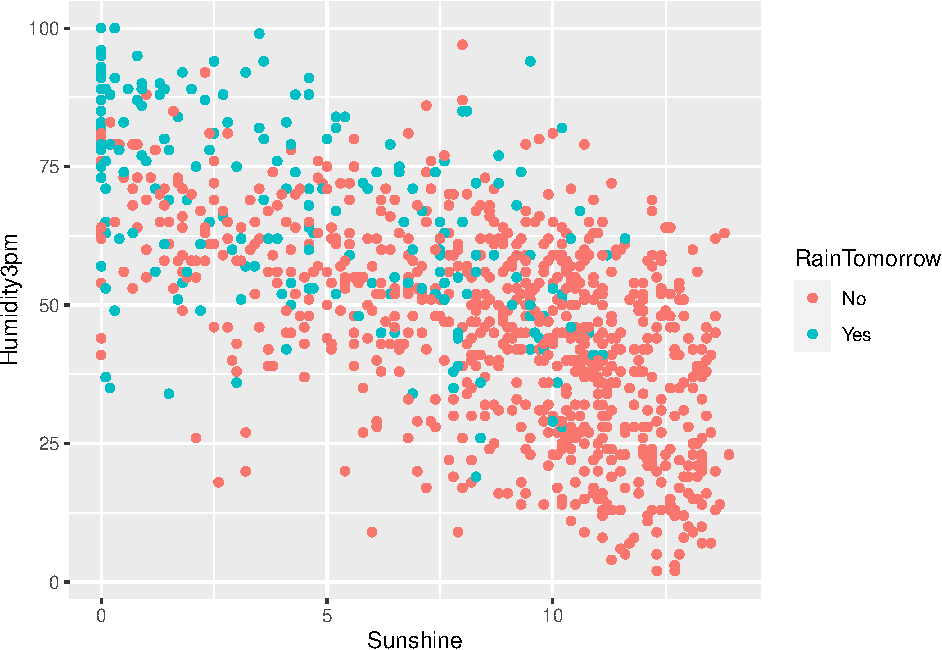
\includegraphics{tpEstadistica_files/figure-latex/unnamed-chunk-10-1.pdf}

\begin{Shaded}
\begin{Highlighting}[]
\NormalTok{ph}\OtherTok{\textless{}{-}}\FunctionTok{ggplot}\NormalTok{(df, }\FunctionTok{aes}\NormalTok{(}\AttributeTok{x=}\NormalTok{Humidity3pm, }\AttributeTok{fill=}\NormalTok{RainTomorrow)) }\SpecialCharTok{+}
  \FunctionTok{geom\_density}\NormalTok{(}\AttributeTok{alpha=}\FloatTok{0.4}\NormalTok{) }\SpecialCharTok{+} \FunctionTok{labs}\NormalTok{(}\AttributeTok{x=} \StringTok{"Nivel de humedad (Humidity3pm)"}\NormalTok{,}
       \AttributeTok{subtitle=}\StringTok{"Grafico densidad humedad"}\NormalTok{) }\SpecialCharTok{+} \FunctionTok{geom\_vline}\NormalTok{(}\AttributeTok{xintercept=}\FloatTok{62.5}\NormalTok{, }\AttributeTok{size=}\FloatTok{0.5}\NormalTok{, }\AttributeTok{color=}\StringTok{"red"}\NormalTok{)}

\NormalTok{ph}
\end{Highlighting}
\end{Shaded}

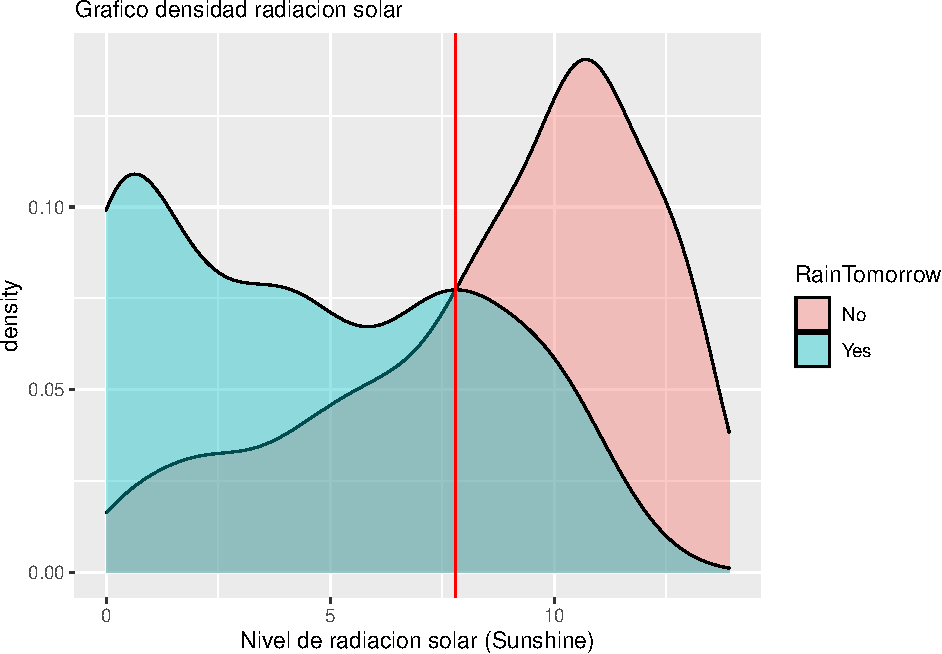
\includegraphics{tpEstadistica_files/figure-latex/unnamed-chunk-11-1.pdf}
Despues de ver estos 2 graficos notamos que no es facil dar un punto de
corte para diferenciar las 2 clases solamente tomando una variable. Ya
que si tomasemos aproximadamente 7.8 de punto de corte para la radiacion
solar o 62 para la humedad como punto de corte, de todas formas tendrias
bastante error ya que las clases se solapan mucho mirandolas
unidimensionalmente. Tomamos estos valores de referencia como para decir
que ningun corte es bueno, estos ni siquiera tienen en cuenta la
diferencia de proporcion de clases. En definitiva no nos casamos con
ninguna variable.

Ejercicio 3. Los boxplot no son buenos graficos. Pueden ocultar
demasiada informacion cuando hoy en dia tenemos la capacidad de
procesarla.

\begin{Shaded}
\begin{Highlighting}[]
\NormalTok{p2}\OtherTok{\textless{}{-}}\FunctionTok{ggplot}\NormalTok{(df, }\FunctionTok{aes}\NormalTok{(}\AttributeTok{y=}\NormalTok{Humidity3pm, }\AttributeTok{x=}\NormalTok{RainTomorrow, }\AttributeTok{fill=}\NormalTok{RainTomorrow)) }\SpecialCharTok{+}
  \FunctionTok{geom\_boxplot}\NormalTok{() }\SpecialCharTok{+} \FunctionTok{labs}\NormalTok{(}\AttributeTok{x=} \StringTok{"Nivel de humedad (Humidity3pm)"}\NormalTok{,}
       \AttributeTok{subtitle=}\StringTok{"Boxplots humedad segun lluvia maniana"}\NormalTok{)}
\NormalTok{p2}
\end{Highlighting}
\end{Shaded}

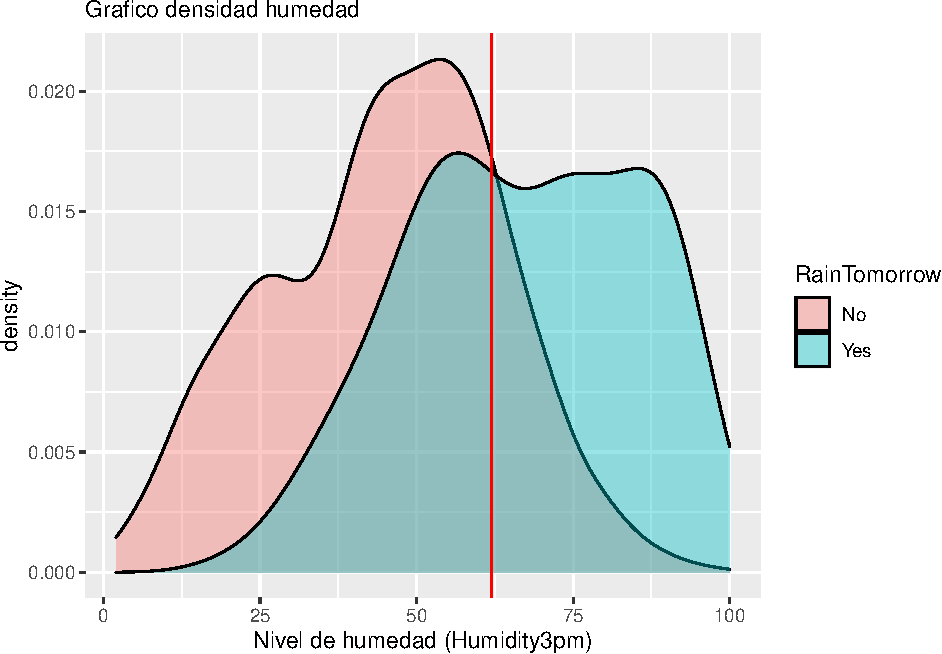
\includegraphics{tpEstadistica_files/figure-latex/unnamed-chunk-12-1.pdf}

\begin{Shaded}
\begin{Highlighting}[]
\NormalTok{p3}\OtherTok{\textless{}{-}}\FunctionTok{ggplot}\NormalTok{(df, }\FunctionTok{aes}\NormalTok{(}\AttributeTok{y=}\NormalTok{Sunshine, }\AttributeTok{x=}\NormalTok{RainTomorrow, }\AttributeTok{fill=}\NormalTok{RainTomorrow)) }\SpecialCharTok{+}
  \FunctionTok{geom\_boxplot}\NormalTok{() }\SpecialCharTok{+} \FunctionTok{labs}\NormalTok{(}\AttributeTok{x=} \StringTok{"Nivel de radiacion solar (Sunshine)"}\NormalTok{,}
       \AttributeTok{subtitle=}\StringTok{"Boxplots radiacion solar segun lluvia maniana"}\NormalTok{)}
\NormalTok{p3}
\end{Highlighting}
\end{Shaded}

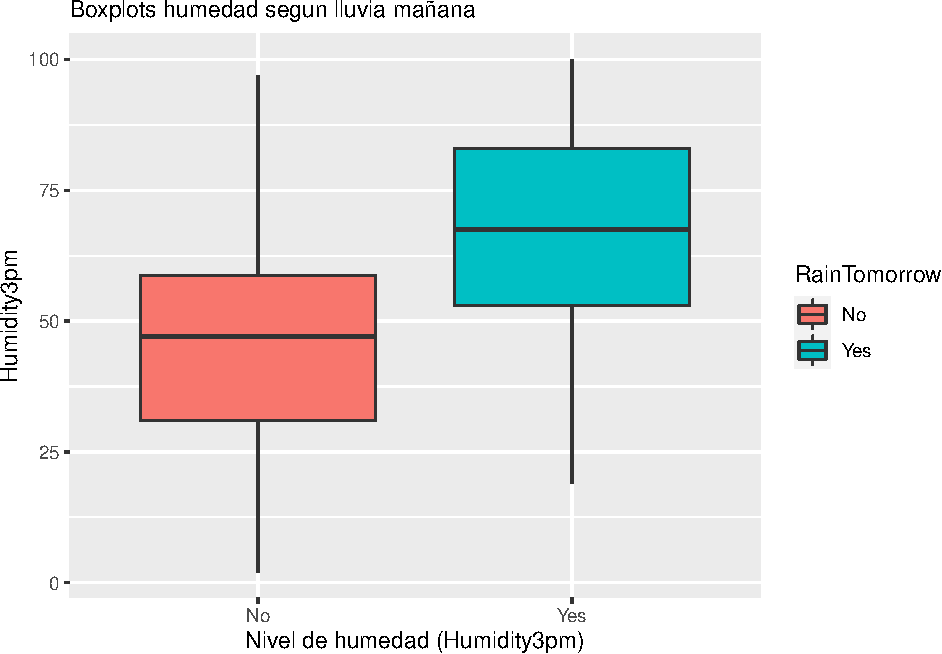
\includegraphics{tpEstadistica_files/figure-latex/unnamed-chunk-13-1.pdf}
Como ven las medias difieren para ambos casos, pero esa informacion ya
la habiamos visto (ademas de muchas otras cosas que aca no) en los
density plots. No hay outliers / valores atipicos.

Ejercicio 4 Para hacer las ventanas moviles voy a primero transformar el
dataset en 1 y 0 a las categoricas, para poder luego tomar promedios.

\begin{Shaded}
\begin{Highlighting}[]
\NormalTok{df}\SpecialCharTok{$}\NormalTok{RainToday }\OtherTok{=} \FunctionTok{ifelse}\NormalTok{(df}\SpecialCharTok{$}\NormalTok{RainToday}\SpecialCharTok{==}\StringTok{"Yes"}\NormalTok{,}\DecValTok{1}\NormalTok{,}\DecValTok{0}\NormalTok{)}
\NormalTok{df}\SpecialCharTok{$}\NormalTok{RainTomorrow }\OtherTok{=} \FunctionTok{ifelse}\NormalTok{(df}\SpecialCharTok{$}\NormalTok{RainTomorrow}\SpecialCharTok{==}\StringTok{"Yes"}\NormalTok{,}\DecValTok{1}\NormalTok{,}\DecValTok{0}\NormalTok{)}
\end{Highlighting}
\end{Shaded}

\begin{Shaded}
\begin{Highlighting}[]
\NormalTok{promediosMoviles }\OtherTok{=} \ControlFlowTok{function}\NormalTok{(datosX, datosY, alturaAestimar, h)\{}
\NormalTok{  df }\OtherTok{=} \FunctionTok{data.frame}\NormalTok{(datosX,datosY)}
\NormalTok{  df2 }\OtherTok{=}\NormalTok{ df[df}\SpecialCharTok{$}\NormalTok{datosX }\SpecialCharTok{\textgreater{}}\NormalTok{ alturaAestimar}\SpecialCharTok{{-}}\NormalTok{h }\SpecialCharTok{\&}\NormalTok{ df}\SpecialCharTok{$}\NormalTok{datosX }\SpecialCharTok{\textless{}}\NormalTok{ alturaAestimar}\SpecialCharTok{+}\NormalTok{h ,]}
  \ControlFlowTok{if}\NormalTok{(}\FunctionTok{mean}\NormalTok{(df2}\SpecialCharTok{$}\NormalTok{datosY)}\SpecialCharTok{\textgreater{}}\DecValTok{1}\SpecialCharTok{/}\DecValTok{2}\NormalTok{ )\{}
    \FunctionTok{return}\NormalTok{(}\DecValTok{1}\NormalTok{)}
\NormalTok{  \}}
  \FunctionTok{return}\NormalTok{(}\DecValTok{0}\NormalTok{)}
\NormalTok{\}}
\end{Highlighting}
\end{Shaded}

\begin{Shaded}
\begin{Highlighting}[]
\FunctionTok{promediosMoviles}\NormalTok{(df}\SpecialCharTok{$}\NormalTok{Sunshine, df}\SpecialCharTok{$}\NormalTok{RainTomorrow, }\DecValTok{8}\NormalTok{, }\FloatTok{0.1}\NormalTok{)}
\end{Highlighting}
\end{Shaded}

\begin{verbatim}
## [1] 0
\end{verbatim}

\begin{Shaded}
\begin{Highlighting}[]
\FunctionTok{promediosMoviles}\NormalTok{(df}\SpecialCharTok{$}\NormalTok{Humidity3pm, df}\SpecialCharTok{$}\NormalTok{RainTomorrow, }\DecValTok{85}\NormalTok{, }\DecValTok{2}\NormalTok{)}
\end{Highlighting}
\end{Shaded}

\begin{verbatim}
## [1] 1
\end{verbatim}

Ejercicio 5 y 6. Nos creamos una funcion que nos genere todo el vector
de predicciones Yhat.

\begin{Shaded}
\begin{Highlighting}[]
\NormalTok{generarColumnaPrediccionesPromediosMoviles }\OtherTok{=} \ControlFlowTok{function}\NormalTok{(datosX, datosY , h)\{}
\NormalTok{  sexoPredicho }\OtherTok{=} \FunctionTok{c}\NormalTok{()}
  \ControlFlowTok{for}\NormalTok{ (i }\ControlFlowTok{in}\NormalTok{ (}\DecValTok{1}\SpecialCharTok{:} \FunctionTok{length}\NormalTok{(datosX)))\{}
\NormalTok{    sexoPredicho[i] }\OtherTok{=} \FunctionTok{promediosMoviles}\NormalTok{(datosX, datosY, (datosX[i]), h)}
\NormalTok{  \}}
  \FunctionTok{return}\NormalTok{(sexoPredicho)}
\NormalTok{\}}
\end{Highlighting}
\end{Shaded}

\begin{Shaded}
\begin{Highlighting}[]
\NormalTok{(}\FunctionTok{generarColumnaPrediccionesPromediosMoviles}\NormalTok{(df}\SpecialCharTok{$}\NormalTok{Sunshine, df}\SpecialCharTok{$}\NormalTok{RainTomorrow, }\DecValTok{1}\NormalTok{))}
\end{Highlighting}
\end{Shaded}

\begin{verbatim}
##    [1] 0 0 0 0 0 0 0 0 0 0 0 0 0 0 0 0 0 0 0 0 0 0 1 0 0 0 1 0 0 0 0 0 0 0 1 1 0
##   [38] 0 0 0 0 0 1 0 0 0 0 0 0 0 0 0 0 0 0 0 0 0 1 0 1 0 0 0 0 0 0 0 0 0 1 0 0 0
##   [75] 0 0 0 0 0 0 0 0 0 0 0 0 0 0 0 0 1 0 0 0 0 0 1 0 0 0 0 0 0 0 0 1 0 1 0 0 0
##  [112] 0 0 0 0 0 0 0 0 0 0 1 0 1 0 0 0 0 0 0 0 0 0 0 1 0 0 0 0 0 1 0 0 0 0 0 0 0
##  [149] 0 0 0 0 0 0 0 1 0 0 0 1 0 0 0 0 0 0 1 0 1 0 0 0 0 0 1 0 0 0 0 0 0 0 0 0 0
##  [186] 0 0 0 0 0 0 0 0 1 0 0 0 0 0 0 0 0 0 0 0 0 0 0 0 0 0 0 0 0 0 1 0 0 0 0 0 0
##  [223] 1 0 0 0 0 0 0 0 0 0 0 0 0 0 0 0 0 0 0 1 0 0 0 1 0 0 0 0 0 0 0 0 0 0 0 0 0
##  [260] 0 0 0 0 0 0 0 0 0 0 0 0 1 1 0 0 0 0 0 0 0 0 0 0 1 0 0 0 0 0 0 0 0 0 0 0 0
##  [297] 0 0 0 0 0 0 0 0 0 0 0 0 0 1 0 1 0 0 0 0 0 0 0 0 0 1 0 0 0 0 0 0 0 0 0 0 0
##  [334] 0 0 0 0 0 0 0 0 0 1 0 0 0 0 0 0 0 0 0 0 0 0 0 0 0 0 0 0 0 0 0 0 0 0 0 0 0
##  [371] 0 0 0 0 0 0 0 0 0 1 0 0 0 0 0 0 0 0 0 0 0 0 0 0 0 0 0 0 0 0 0 0 0 0 0 0 0
##  [408] 1 0 0 0 0 1 0 0 0 0 0 0 0 0 0 0 0 0 0 0 0 1 0 0 0 0 0 0 0 0 0 0 0 0 0 0 0
##  [445] 0 0 1 0 0 0 0 0 0 0 0 1 0 0 0 0 0 0 0 0 0 0 1 0 0 0 0 0 0 0 0 0 0 0 0 0 0
##  [482] 0 0 1 0 1 0 0 0 0 0 0 0 0 0 0 0 0 0 1 0 0 0 0 0 0 0 0 0 0 0 0 0 0 0 0 0 0
##  [519] 0 0 0 0 0 1 0 0 1 0 0 0 0 0 0 0 0 0 0 0 0 0 0 0 0 1 0 0 0 0 0 0 0 0 0 0 0
##  [556] 0 0 1 0 0 0 0 1 0 0 0 0 0 0 0 0 0 0 0 0 0 0 0 0 0 0 0 0 0 0 0 0 0 0 0 0 0
##  [593] 0 0 0 1 0 0 0 0 0 0 0 0 0 0 0 0 0 0 0 0 0 0 0 0 0 0 0 0 0 0 0 0 0 0 0 0 0
##  [630] 0 0 0 0 0 0 0 0 0 0 0 0 0 0 0 0 0 0 0 0 0 0 0 0 0 0 0 0 0 0 0 1 1 0 0 1 0
##  [667] 0 0 0 1 0 0 0 0 0 0 0 0 0 0 0 1 0 0 0 0 0 0 1 0 0 0 0 1 0 0 0 0 0 0 0 0 0
##  [704] 0 0 0 0 0 0 0 0 0 0 0 0 0 0 0 0 0 0 0 0 0 0 0 0 0 0 0 0 0 0 0 1 0 0 0 0 0
##  [741] 1 0 0 0 0 0 0 0 0 0 1 0 0 0 0 0 0 0 0 0 0 0 0 1 0 0 0 0 0 0 0 0 0 0 0 1 0
##  [778] 1 0 0 0 0 0 0 0 0 0 0 0 0 1 1 0 0 0 0 0 0 0 0 0 0 0 0 0 0 0 0 1 0 0 0 1 0
##  [815] 0 0 0 0 0 0 0 0 0 0 0 0 0 0 0 0 0 0 0 0 0 0 0 0 0 1 0 0 0 0 1 0 0 0 0 0 0
##  [852] 0 0 0 0 0 1 0 0 0 0 0 0 0 0 0 0 1 0 0 0 0 0 0 0 0 0 0 1 0 1 0 0 0 0 0 0 0
##  [889] 0 0 0 0 0 0 0 0 0 1 0 0 0 0 0 0 0 0 0 0 1 0 0 0 0 0 0 0 0 0 1 0 0 0 0 0 0
##  [926] 0 1 1 0 0 0 0 0 0 0 0 0 0 0 0 0 0 0 0 0 0 0 0 0 0 0 0 0 0 0 0 0 0 0 0 0 0
##  [963] 0 0 1 0 0 0 0 1 0 0 0 0 0 0 0 0 1 0 0 0 0 0 0 0 0 0 0 0 0 0 0 0 0 0 0 0 0
## [1000] 0
\end{verbatim}

Vamos a evaluarlo con el metodo de validacion cruzada de LOO (dejar uno
afuera para entrenar y evaluarlo con ese).

\begin{Shaded}
\begin{Highlighting}[]
\NormalTok{leaveOneOut }\OtherTok{=} \ControlFlowTok{function}\NormalTok{(datosX, datosY, h)\{}
\NormalTok{  error }\OtherTok{=} \DecValTok{0}
  \ControlFlowTok{for}\NormalTok{ (i }\ControlFlowTok{in}\NormalTok{ (}\DecValTok{1}\SpecialCharTok{:} \FunctionTok{length}\NormalTok{(datosX)))\{}
\NormalTok{    predichoI }\OtherTok{=} \FunctionTok{promediosMoviles}\NormalTok{(df}\SpecialCharTok{$}\NormalTok{Sunshine[}\SpecialCharTok{{-}}\NormalTok{i], df}\SpecialCharTok{$}\NormalTok{RainTomorrow[}\SpecialCharTok{{-}}\NormalTok{i], df}\SpecialCharTok{$}\NormalTok{Sunshine[i], h)}
\NormalTok{    error }\OtherTok{=}\NormalTok{ error }\SpecialCharTok{+} \FunctionTok{abs}\NormalTok{(predichoI }\SpecialCharTok{{-}}\NormalTok{ df}\SpecialCharTok{$}\NormalTok{RainTomorrow[i])}
\NormalTok{  \}}
  \FunctionTok{return}\NormalTok{(error)}
\NormalTok{\}}
\end{Highlighting}
\end{Shaded}

\begin{Shaded}
\begin{Highlighting}[]
\NormalTok{hPosibleHumedad }\OtherTok{=} \FunctionTok{seq}\NormalTok{(}\FloatTok{0.2}\NormalTok{, }\DecValTok{10}\NormalTok{, }\FloatTok{0.8}\NormalTok{ )}
\NormalTok{hPosibleSunshine }\OtherTok{=} \FunctionTok{seq}\NormalTok{(}\FloatTok{0.5}\NormalTok{, }\DecValTok{4}\NormalTok{, }\FloatTok{0.1}\NormalTok{ )}
\end{Highlighting}
\end{Shaded}

\begin{Shaded}
\begin{Highlighting}[]
\NormalTok{erroreshHumedad }\OtherTok{=} \FunctionTok{c}\NormalTok{()}
\ControlFlowTok{for}\NormalTok{ (i }\ControlFlowTok{in}\NormalTok{ (}\DecValTok{1}\SpecialCharTok{:} \FunctionTok{length}\NormalTok{(hPosibleHumedad)))\{}
\NormalTok{    erroreshHumedad[i] }\OtherTok{=} \FunctionTok{leaveOneOut}\NormalTok{(df}\SpecialCharTok{$}\NormalTok{Humidity3pm, df}\SpecialCharTok{$}\NormalTok{RainTomorrow, hPosibleHumedad[i])}
\NormalTok{\}}
\end{Highlighting}
\end{Shaded}

\begin{Shaded}
\begin{Highlighting}[]
\NormalTok{erroreshSunshine }\OtherTok{=} \FunctionTok{c}\NormalTok{()}
\ControlFlowTok{for}\NormalTok{ (i }\ControlFlowTok{in}\NormalTok{ (}\DecValTok{1}\SpecialCharTok{:} \FunctionTok{length}\NormalTok{(hPosibleSunshine)))\{}
\NormalTok{    erroreshSunshine[i] }\OtherTok{=} \FunctionTok{leaveOneOut}\NormalTok{(df}\SpecialCharTok{$}\NormalTok{Sunshine, df}\SpecialCharTok{$}\NormalTok{RainTomorrow, hPosibleSunshine[i])}
\NormalTok{\}}
\end{Highlighting}
\end{Shaded}

\begin{Shaded}
\begin{Highlighting}[]
\FunctionTok{plot}\NormalTok{(hPosibleHumedad , erroreshHumedad, }\AttributeTok{type =} \StringTok{"l"}\NormalTok{)}
\end{Highlighting}
\end{Shaded}

\includegraphics{tpEstadistica_files/figure-latex/unnamed-chunk-24-1.pdf}
De aca vemos que la ventana optima para humedad es de exactamente 1.

\begin{Shaded}
\begin{Highlighting}[]
\FunctionTok{plot}\NormalTok{(hPosibleSunshine , erroreshSunshine, }\AttributeTok{type =} \StringTok{"l"}\NormalTok{)}
\end{Highlighting}
\end{Shaded}

\includegraphics{tpEstadistica_files/figure-latex/unnamed-chunk-25-1.pdf}
Mientras que la ventana optima para la radiacion solar es de 0.8

Asi el error de clasificacion empirico despues de encontrar el h optimo
para sunshine es de 179. Es decir le erra el 17.9\% de las veces

\end{document}
